% Copyright (c) 2012 University of Pennsylvania. All rights reserved.
% See http://www.rad.upenn.edu/sbia/software/license.html or COPYING file.
%
% Contact: SBIA Group <sbia-software at uphs.upenn.edu>

\documentclass[a4paper,12pt]{article}

\usepackage{cite}
\usepackage{geometry}
\usepackage{graphicx}
\usepackage{subfigure}
\usepackage{hyperref}
\usepackage{url}

\usepackage[cm]{fullpage}

\usepackage{fancyvrb}
\usepackage{color}

\usepackage[usenames,dvipsnames]{xcolor}
\definecolor{light-gray}{gray}{0.95}
\newcommand{\tabincell}[2]{\begin{tabular}{@{}#1@{}}#2\end{tabular}}


% Title Page
\title{DRAMMS Software Flyer}
\author{Yangming Ou, Andreas Schuh}

\begin{document}
\maketitle
% \tableofcontents
% \setcounter{tocdepth}{1}

% \pagebreak

% ============================================================================
% Introduction
% ============================================================================
\section{Introduction}
\label{intro}

DRAMMS is a deformable image registration software package designed for 2D-to-2D and 3D-to-3D image registrations. Fig. \ref{fig:DRAMMSApplications} shows some typical applications, including, 

\indent -- Cross-subject registration of the same organ (brain, breast, cardiac, etc); \\
\indent -- Mono- and Multi-modality registration (MRI, CT, histology); \\
\indent -- Longitudinal registration (pediatric brain growth, cancer development, etc); \\
\indent -- Registration under partial missing correspondences (small lesions, tumors, histological cuts). \\


\begin{figure}[ht!]
	\centering
	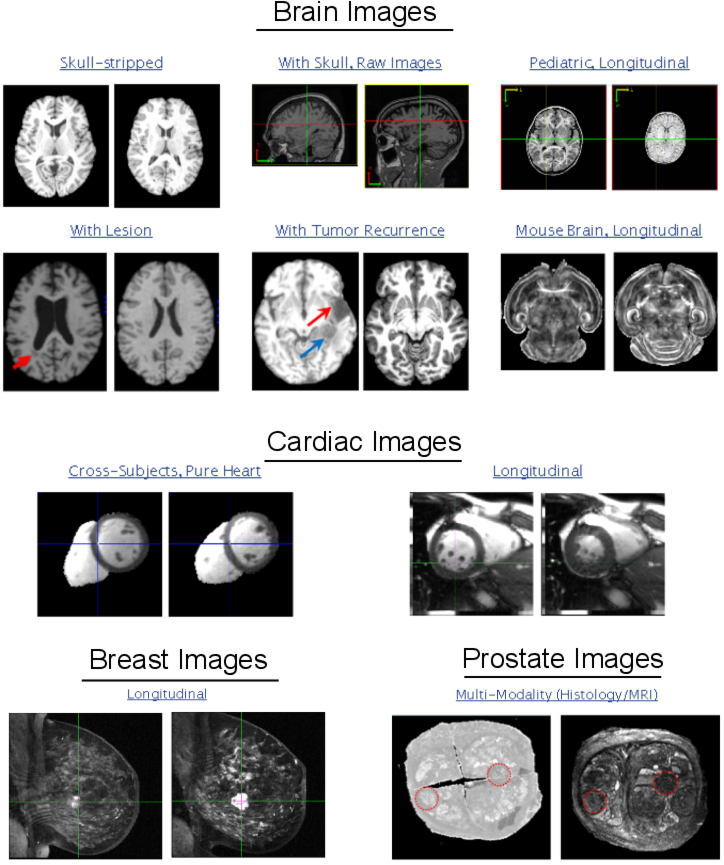
\includegraphics[width=15cm]{AllExamples.png}
	\caption{Some typical DRAMMS applications.}
	\label{fig:DRAMMSApplications}
\end{figure}

\noindent {\bf{DRAMMS Homepage:}} \url{http://www.rad.upenn.edu/sbia/software/dramms/index.html} \\
\noindent {\bf{DRAMMS Manual:}} \url{http://www.rad.upenn.edu/sbia/software/dramms/_downloads/DRAMMS_Software_Manual.pdf} 



\section{System Requirement}  
\label{System}  

\noindent {\bf{OS:}} UNIX/LINUX or Mac. \\
\noindent {\bf{File formats:}} ANALYZE 7.5 (.hdr+.img) or NIfTI-1 (.hdr+.img, .nii, .nii.gz) images. \\
\noindent {\bf{Datatypes:}} byte, uint8, int8, short, int16, uint16, float, float32, int32. \\
\noindent {\bf{Memory:}} DRAMMS consumes considerable amount of memory ($\sim$50MB for 2D images, and $\sim$6GB for a typical pair of brain MR images $256\times256\times150$). \\


\section{Download and Install}
\label{install}

{\bf{Download:}} \url{http://www.rad.upenn.edu/sbia/software/dramms/download.html}. \\
{\bf{Install :}} \url{http://www.rad.upenn.edu/sbia/software/dramms/installation.html}. Requires CMake (version 2.8 or above) and GCC (version 4.1 or above).




\section{Usage}
\label{usage}
Default usage below will get reasonable results in most cases. 
\begin{verbatim}
    dramms -S ${SourceImage}         -T ${TargetImage} 
           -O ${RegisteredImage_S2T} -D ${Deformation_S2T} 
\end{verbatim}
More specific usage including parameter tuning in various scenarios can be found in Tutorial page \url{http://www.rad.upenn.edu/sbia/software/dramms/tutorials.html}.





\begin{thebibliography}{4}

\bibitem{Ou11} Yangming Ou, Aris Sotiras, Nikos Paragios, Christos Davatzikos: DRAMMS: Deformable registration via attribute matching and mutual-saliency weighting. Medical Image Analysis 15(4): 622-639 (2011).


\end{thebibliography}


% ============================================================================
% Bibliography
% ============================================================================
\bibliographystyle{splncs03}
\bibliography{references}

\end{document}          
